%LLMs, trained on trillions of tokens with billions of parameters have shown unparalleled capabilities in a wide range of natural language processing tasks~\cite{}. Nevertheless, significant attention have drawn from both the research community and industry on the concerns about their precision, complex reasoning, and planning capabilities ~\cite{}. While advanced prompting approaches such as Chain, Tree, Graph-of-Thought~\cite{}, which generate intermediate steps in the reasoning process demonstrate large improvements on reasoning capability of LLMs, it remains essential to fine-tune LLMs using a substantial volume of high-quality, supervised data to fundamentally improve the model performance~\cite{}. This methodology is inherently limited by the scope and quality of data that humans can provide~\cite{}.

% @article{huang2023large,
%   title={Large language models cannot self-correct reasoning yet},
%   author={Huang, Jie and Chen, Xinyun and Mishra, Swaroop and Zheng, Huaixiu Steven and Yu, Adams Wei and Song, Xinying and Zhou, Denny},
%   journal={arXiv preprint arXiv:2310.01798},
%   year={2023}
% }

% @inproceedings{clark2015training,
%   title={Training deep convolutional neural networks to play go},
%   author={Clark, Christopher and Storkey, Amos},
%   booktitle={International conference on machine learning},
%   pages={1766--1774},
%   year={2015},
%   organization={PMLR}

% @article{valmeekam2022large,
%   title={Large language models still can't plan (a benchmark for llms on planning and reasoning about change)},
%   author={Valmeekam, Karthik and Olmo, Alberto and Sreedharan, Sarath and Kambhampati, Subbarao},
%   journal={arXiv preprint arXiv:2206.10498},
%   year={2022}
% }
% @article{stechly2024self,
%   title={On the Self-Verification Limitations of Large Language Models on Reasoning and Planning Tasks},
%   author={Stechly, Kaya and Valmeekam, Karthik and Kambhampati, Subbarao},
%   journal={arXiv preprint arXiv:2402.08115},
%   year={2024}
% }

LLMs, trained on trillions of tokens with billions of parameters have shown unparalleled capabilities in a wide range of natural language processing tasks~\citep{touvron2023llama,team2023gemini,openai2023gpt}. Nevertheless, they continue to face challenges in scenarios requiring complex reasoning and strategic planning ~\citep{valmeekam2022large,stechly2024self}. While advanced prompting approaches such as Chain, Tree, Graph-of-Thought~\citep{wei2022chain,yao2024tree, besta2024graph, ding2023everything}, it remains essential to fine-tune LLMs using a substantial volume of high-quality, supervised data to fundamentally improve the model performance~\citep{nye2021show,lewkowycz2022solving,chung2022scaling}. This methodology is inherently limited by the scope and quality of data that humans can provide.

% LLMs, trained on trillions of tokens with billions of parameters have shown unparalleled capabilities in a wide range of natural language processing tasks~\citep{touvron2023llama,team2023gemini,openai2023gpt}. Nevertheless, they continue to face challenges in scenarios requiring complex reasoning and strategic planning ~\citep{valmeekam2022large,stechly2024self}. While advanced prompting approaches such as Chain, Tree, Graph-of-Thought~\citep{wei2022chain,yao2024tree, besta2024graph, ding2023everything}, which generate intermediate steps in the reasoning process demonstrate large improvements on reasoning capability of LLMs, it remains essential to fine-tune LLMs using a substantial volume of high-quality, supervised data to fundamentally improve the model performance~\citep{nye2021show,lewkowycz2022solving,chung2022scaling}. This methodology is inherently limited by the scope and quality of data that humans can provide.

Considering these challenges, the concept of self-correction and self-learning have been proposed as promising solutions~\citep{madaan2024self,saunders2022self,chen2024self}. Within these framework, LLMs typically operate by employing two main strategies: 1) they continuously refine their responses based on the feedback of their past responses, and 2) they extensively sample responses then learn from preferences judged by itself as reward models with PPO or DPO~\citep{yuan2024advancing,yuan2024self,chen2024self}. However, it remains a matter of ongoing research whether LLMs can effectively critique their own outputs to either enhance response quality or apply a scalar reward to indicate the quality of responses, especially in contexts demanding intricate planning and reasoning~\citep{valmeekam2022large,stechly2024self,huang2023large,hong2023closer}. On the other hand, advanced search algorithms such as MCTS, combined with reinforcement learning, have enabled models to learn from self-play and achieve human parity or even surpass human performance in complex tasks such as the game of Go~\citep{silver2016mastering, silver2017mastering}. This naturally raises a question: is it viable to leverage the strengths of MCTS alongside LLMs to inaugurate a novel paradigm of self-improving? More precisely, could the assimilation of MCTS empower LLMs to more effectively explore better responses, guided by strategic signals, and subsequently optimize these responses to enhance overall performance?

% To answer this question, we firstly take a systematic view of AlphaGo. There are three key elements lead to the success of it: 1) Large volume of expert and self-playing data; The imitation learning on expert data allows it to learn and mimic human-like moves, and the learning on self-play data encourages the discovery of innovative tactics beyond human limitations~\citep{clark2015training}. 2) MCTS that helps explore possible moves based on statistical sampling of the search space. By efficiently narrowing down the most promising moves and simulating their outcomes, AlphaGo could make highly informed decisions even in the complex and vast decision space. 3) Accurate and distinct environment feedback; The clear and accurate feedback (win or loss) from the environment in Go provided AlphaGo with a straightforward and unambiguous signal to learn from. Taking these key elements into considerations, the integration of MCTS for LLM self-improving introduces several challenges: 1) Limited Data: The high-quality annotation data for LLMs is typically limited.  In addition, the synthesis of effective training data for LLMs, akin to AlphaGo's self-play, remains a research question. 2) Search efficiency: The potential token combinations in natural language tasks create an exponentially large search space, presenting a formidable obstacle to the efficiency of MCTS. 3) Imperfect feedback: Unlike the clear win/loss signal in Go, feedback in natural language tasks is often subjective and nuanced, lacking a straightforward metric for success. 

To answer this question, we begin with a systematic examination of AlphaGo, identifying three critical aspects for its success: (\RN{1}) The large volume of data, including self-play data. (\RN{2}) The use of tree search, which facilitates the exploration of potential moves through statistical sampling of the large search space. (\RN{3}) Accurate and unambiguous environment feedback; the direct and accurate feedback (win or loss) provided by the game of Go offers a clear and unequivocal learning signal~\citep{silver2017mastering}. The integration of MCTS with LLMs for self-improvement has several challenges: (\RN{1}) Limited Data: High-quality annotated data for LLMs is generally scarce. Furthermore, how to construct of synthetic data for LLMs training, similar to AlphaGo's self-play data, remains unclear. (\RN{2}) Search Efficiency: The vast number of potential token combinations in natural language tasks results in an exponentially large search space, posing a significant challenge to the efficiency of MCTS~\citep{Ramamurthy2022IsRL}. (\RN{3}) Imperfect Feedback: In contrast to the clear win/loss feedback in Go, feedback in natural language tasks is often subjective and nuanced, without a straightforward measure of success.

% To answer this question, we begin with a systematic examination of AlphaGo, identifying three critical aspects for its success: (\RN{1}) The large volume of expert and self-play data; imitation learning on expert data enables it to simulate human-like strategies, and the reinforcement learning on self-play data fosters the emergence of novel tactics that surpass human capabilities~\citep{clark2015training}. (\RN{2}) The use of tree search, which facilitates the exploration of potential moves through statistical sampling of the large search space. This approach allows AlphaGo to effectively identify and simulate the most promising strategies, thereby making highly informed decisions in the complex and vast decision space~\citep{silver2016mastering}. (\RN{3}) Accurate and unambiguous environment feedback; the direct and accurate feedback (win or loss) provided by the game of Go offers a clear and unequivocal learning signal~\citep{silver2017mastering}. The integration of MCTS with LLMs for self-improvement has several challenges: (\RN{1}) Limited Data: High-quality annotated data for LLMs is generally scarce. Furthermore, how to construct of synthetic data for LLMs training, similar to AlphaGo's self-play data, remains unclear. (\RN{2}) Search Efficiency: The vast number of potential token combinations in natural language tasks results in an exponentially large search space, posing a significant challenge to the efficiency of MCTS~\citep{Ramamurthy2022IsRL}. (\RN{3}) Imperfect Feedback: In contrast to the clear win/loss feedback in Go, feedback in natural language tasks is often subjective and nuanced, without a straightforward measure of success.

\begin{figure}[!t]
    \centering
    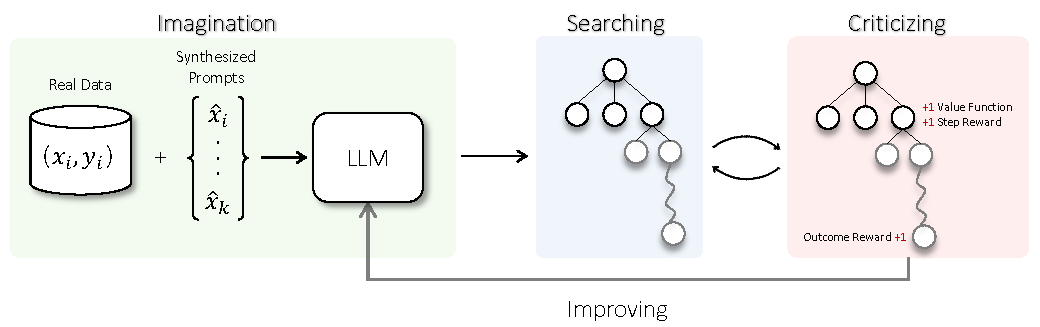
\includegraphics[width=0.9\textwidth]{figures/framework_crop.pdf}
    \caption{Imagination-Searching-Criticizing self-improvement loop: Imagination component synthesizes prompts as new learning examples, with MCTS searching better trajectories guided by signals from critics for policy improving.}
    \label{fig:framework}
\end{figure}

In this paper, we introduce \model{}, an imagination-searching-criticizing framework designed for the self-improvement of LLMs . \model{} consists of three key components, as illustrated in Figure~\ref{fig:framework}. First, an imagination component is designed to synthesize prompts, alleviating the issues of data scarcity. Second, we propose \emcts{} tailored for efficient searching in language tasks. Particularly, it has been show that planning at multiple levels of temporal abstraction is critical for RL problems with a long horizon and large action space~\citep{sutton1999between,peng2017composite,Luketina2019ASO}. As such, we propose formulating the text generation process as options over a Markov Decision Process (MDP) problem, where each option represents the generation of a collection of tokens for a specific subtask, similar to the concept of chains in chain-of-thought prompting. This formulation improves search efficiency by substantially reducing the search depth. Additionally, we propose the use of state merge and adaptive branching factors to further enhance search efficiency by balancing the trade-off between search width and depth. Lastly, since accurate feedback is crucial to the success of MCTS, we introduce a trio of critic models to guide \emcts{}, including a value function for estimating expected rewards, a process reward model for assessing node correctness, and an outcome reward model for evaluating the overall trajectory. For complex tasks with which LLMs struggle assessing such as arithmetic computation and code execution, to ensure the accuracy of feedback, we augment the critics with the capacity to make dynamic decisions on which tools to use, when to use them, and how to use them effectively. After \emcts{} stage, we collect the trajectory with the largest reward from the critic models as the training examples to improve LLMs. 

The experimental results on mathematical reasoning tasks demonstrate that \model{} can efficiently search for better responses and use them to improve LLMs' performance, forming an effective self-improving loop. Notably, based on Llama-2-70b and WizardMath-70B-V1.0, \model{} can improve its performance from 57.8 to 92.0 on GSM8K and from 20.7 to 51.0 on MATH, performing comparably to GPT-4. 

% In summary, our contributions are threefold:
% \begin{itemize}
% \item We examine the inherent challenges in harnessing AlphaGo's self-learning algorithms for LLMs, which are data scarcity, the complexity of search spaces, and the nuanced nature of feedback.
% \item We introduce \model{}, an imagination-searching-criticizing framework that integrates MCTS with LLMs, enabling them to self-improve without the need for additional annotations
% \item Experiments on mathematical reasoning problems show that, by employing \model{}, we can significantly enhance the performance of LLaMA-2 70B, elevating it to levels comparable with GPT-4 on the GSM8K and MATH datasets when \emcts{} decoding is utilized.
% \end{itemize}
% \begin{itemize}\setlength{\itemsep}{0pt}
% \item We analyze the challenges of applying AlphaGo style self-learning algorithm to LLMs and introduce \model{}, a novel framework that synergizes MCTS with LLMs for self-improvement.
% \item We integrate
% \item Experimental results on mathematical reasoning showcases remarkable performance gains of using MCTS for self-improving, validating the efficacy of \model{}.
% \end{itemize}


% propose to improve MCTS efficiency by formulating the task as options over MDPs problems. This formulation improves search efficiency by utilizing options, which are temporal abstractions of multiple tokens, rather than a single token as the search nodes. Additionally, techniques such as state fusion and adaptive branching factors are implemented to improve search efficiency by balancing the trade-off between search breadth and depth. 


% \begin{itemize}
%     \item LLM
%     \item LLM struggles at planning (left-to-right next token prediction)
%     \item AlphaX + LLM has several challenges
%     \item AlphaX: Action is clearly defined; Signal is 100\% accurate;
%     \item AlphaX + LLM:
%     \item Search
%     \begin{itemize}
%         \item Step: Options over MDP
%         \item Signal: Specialized statistical model + Symbolic engines (fast-rollout)
%         \item Efficient MCTS: state merger, adaptive exploration
%         \item slow/fast thinking ()
%     \end{itemize}
%     \item Learning
% \end{itemize}